\begin{figure*}
    \centering 
    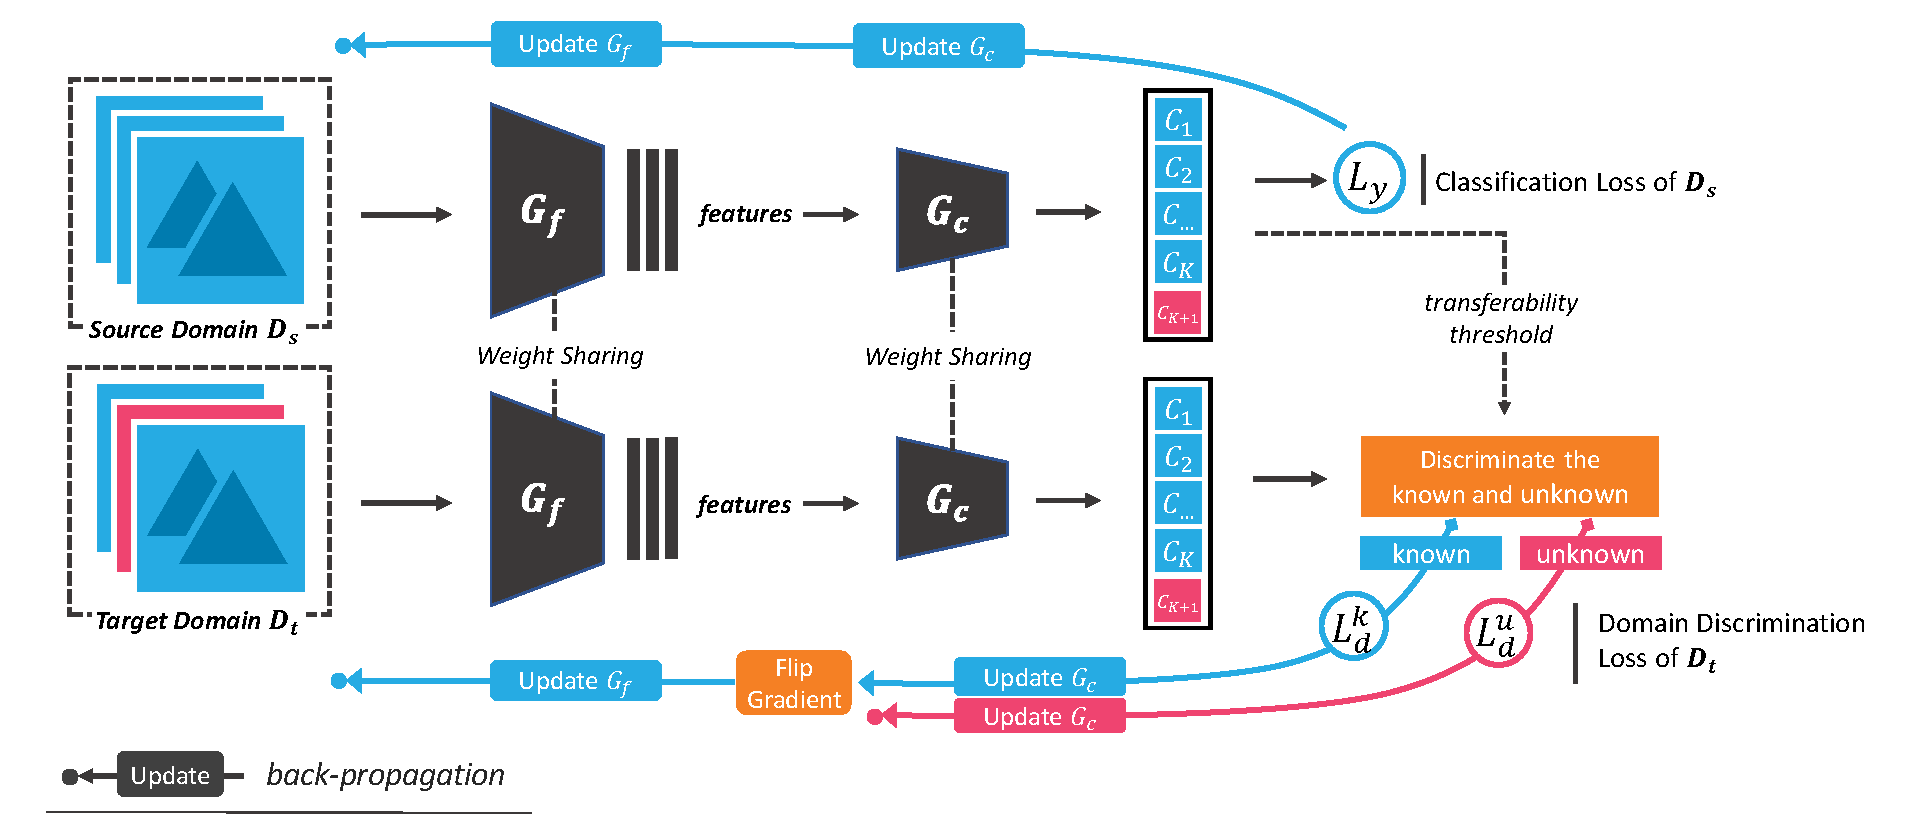
\includegraphics[width=0.95\textwidth]{contents/figures/pdf/ThDANN.pdf} 
    \caption{
        The network architecture of the proposed Thresholded Domain Adversarial Network \textit{\textbf{(ThDAN)}}. The classifier $G_C$ output $K+1$ dimensional probabilistic output after the $G_f$ extract features. For source samples, the $G_c$ and $G_f$ are trained to correctly classify them by minimizing classification loss $L_y$. For the target samples, we begin with splitting them into the known class partition and the unknown class partition according to \figurename{\ref{figure: selection}}, then calculate domain discriminate loss $L_d$ for this two partition respectivly. By minimizing $L_d$ to update $G_c$, we can correctly label the unknown class samples. In the aid of the gradient reversal layer (GRL), we can use $L_d$ to update $G_f$ to match the distribution between the known-marked samples and the samples of source domain.
    } 
    \label{figure: ThDANN} 
\end{figure*}